\documentclass[12pts]{beamer}
\usepackage[utf8]{inputenc}
\usepackage[T1]{fontenc}
\usepackage[spanish]{babel}

\usepackage{graphicx}
\usepackage{apacite}
\usepackage{amsfonts, amsmath, amssymb}
\usepackage{physics, units}
\usepackage{listings}
\usepackage{tikz}

\usetheme{Marburg}
\usecolortheme{crane}

\setbeamertemplate{background}{
	\tikz\node[opacity=0.4, inner sep=0pt] {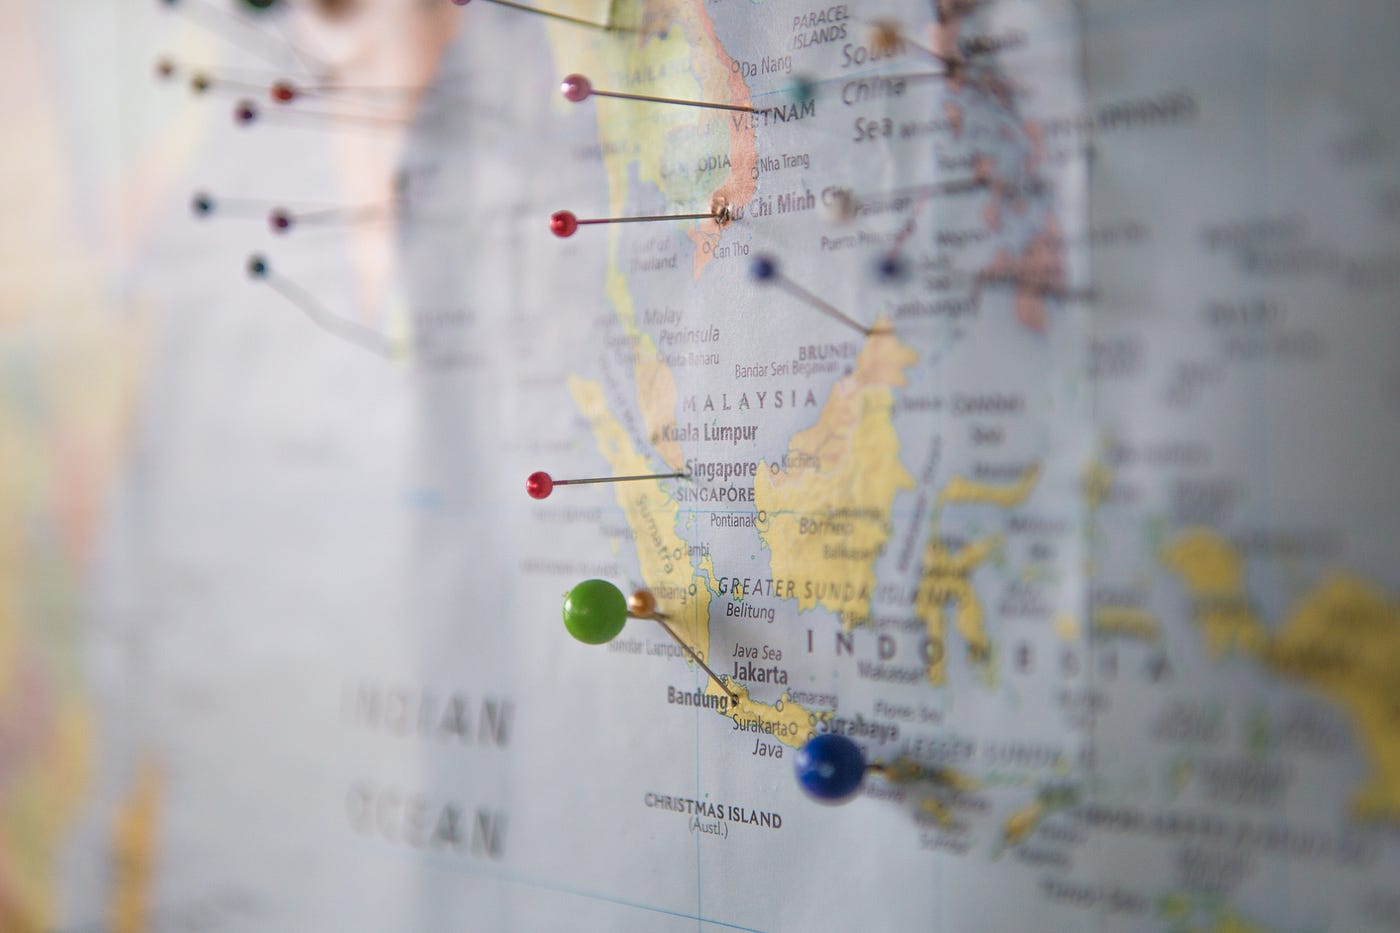
\includegraphics[width=\paperwidth,height=\paperheight]{geographic_statistics_background.jpg}};}

\definecolor{aliceblue}{rgb}{0.94, 0.97, 1.0}
\definecolor{amethyst}{rgb}{0.6, 0.4, 0.8}
\definecolor{aqua}{rgb}{0.6, 0.99, 0.99}
\definecolor{mygray}{rgb}{0.93, 0.99, 0.97}
\definecolor{arsenic}{rgb}{0.23, 0.27, 0.29}
\definecolor{ballblue}{rgb}{0.13, 0.67, 0.8}
\definecolor{blue-green}{rgb}{0.0, 0.87, 0.87}

\setbeamertemplate{sidebar canvas right}[vertical shading][top=aqua, bottom=mygray] 

\setbeamercolor{palette primary}{fg=aliceblue, bg=orange}
\setbeamercolor{palette secondary}{fg=arsenic, bg=white}
\setbeamercolor{palette tertiary}{fg=aqua}
\setbeamercolor{palette quaternary}{fg=ballblue, bg=mygray}

\setbeamertemplate{footline}
{
  \leavevmode%
  \hbox{%
    \begin{beamercolorbox}[wd=.30\paperwidth,ht=2.25ex,dp=1ex,center]{author in head/foot}%
      \usebeamerfont{author in head/foot}\insertshortauthor%~~(\insertshortinstitute)
    \end{beamercolorbox}%
    \begin{beamercolorbox}[wd=.40\paperwidth,ht=2.25ex,dp=1ex,center]{title in head/foot}%
      \usebeamerfont{title in head/foot}\insertshortsubtitle
    \end{beamercolorbox}%
    \begin{beamercolorbox}[wd=.30\paperwidth,ht=2.25ex,dp=1ex,center]{date in head/foot}%
      \usebeamerfont{date in head/foot}\periodo{}\hspace*{2em}
      \usebeamertemplate{page number in head/foot}\hspace*{4ex}
    \end{beamercolorbox}
  }%
  \vskip0pt%
}

\AtBeginDocument{\renewcommand\refname{Bibliografía}}
\global\newcommand{\periodo}{\textit{I-PAC 2024}}
%\periodo{IIIPAC}

\author[Facultad de Ciencias - UNAH]{\color{arsenic}{\textit{\textbf{J. Moisés Arias}}}}
\title{\color{arsenic}{\textbf{Técnicas de Muestreo Espacial: Aplicaciones e Implementación en R}}}
\subtitle{\color{black}{\textbf{Teoría de Muestreo MM535}}}
\date{Abril, 2024}


\begin{document}
	
	\begin{frame}
		\maketitle
	\end{frame}

	\begin{frame}{Contenidos}
		\tableofcontents
	\end{frame}

	\section{Introducción}
	\begin{frame}{Introducción}
		Las poblaciones cuyas observaciones varían según su distribución geográfica ameritan una colección de técnicas especiales para su análisis.\\[1cm]
		
		Dichas técnicas son de gran importancia en geología, meteorología, ecología y ciencias sociales. Se conocen como muestreo espacial.
	\end{frame}

	\section{Objetivos}
	\begin{frame}{Objetivos}
	\begin{itemize}
		\item \textbf{Objetivo General}\\
		Ampliar los conocimientos sobre las técnicas de muestreo de una población  distribuida en una región geográfica. 
		\item \textbf{Objetivos específicos}	
		\begin{enumerate}
			\item Integrar los modelos de muestreo básicos en el contexto de una muestra espacialmente variable. 
			\item Conocer las aplicaciones del muestreo espacial. 
			\item Implementar los métodos de muestreo espacial en R. 
		\end{enumerate}
	\end{itemize}
¸	\end{frame}

	\section{Breve reseña histórica}
	\begin{frame}{Breve reseña histórica}
	La aplicación de la estadística para recoger y analizar información sobre regiones geográficas ha cobrado mayor importancia en la actualidad.\\[1cm]
	
	La geoestadística fue desarrollada para analizar datos geológicos distribuidos en el espacio de un cuerpo mineral. Sus principales proponentes, habrían sido Matheron, Whittle y Gandin.
	\end{frame}

	\subsection{Utilidad y aplicaciones}
	\begin{frame}{Utilidad y aplicaciones}
		Los métodos de muestreo espacial se aplican a:
		\begin{enumerate}
			\item el manejo de recursos agrícolas y forestales.
			\item predicción de reservas minerales y fósiles.
			\item monitoreo de especímenes en una región.
			\item rastreo de la propagación de una infección en una localidad. 
		\end{enumerate}
	\end{frame}

	\section{Predicción espacial: kriging}
	\begin{frame}{Muestreo espacial}
		En el muestreo espacial se contemplan cantidades ambientales, ecológicas o geológicas como una variable aleatoria  $y_t$ cuyos valores son observaciones de un proceso estocástico
		
		\begin{equation}
		\left\lbrace y_t : t \in D \subset \mathbb{R}^d \right\rbrace\label{proceso}
		\end{equation}
		
	\end{frame}
	
	\begin{frame}{Generalidades del kriging}
		\begin{itemize}
			\item Los modelos muestrales tradicionales son inadecuados.
			\item Kriging no realiza estimaciones, sino predicciones. 
			\item El fin del kriging es predecir una variable aleatoria $y_0$ en una región desconocida.
			\item El predictor de kriging es insesgado y de varianza mínima.
		\end{itemize}
	\end{frame}

	\begin{frame}{Tipos de kriging}
		\begin{itemize}
			\item Kriging simple: se conoce $\mu_i$ y $Cov(y_i, y_j)$.
			\item Kriging ordinario: se conoce $\mu_i$, se estima $Cov(y_i, y_j)$. 
			\item Kriging universal: se estima $\mu_i$, se conoce $Cov(y_i, y_j)$.
		\end{itemize}
	\end{frame}

	\begin{frame}{Modelo genérico}
		\begin{align}
		y_t =& \mu_t +\epsilon_t\\
		\epsilon_t \sim& \mathcal{N}(0, \sigma^2)\\
		Cov(\epsilon_t, \epsilon_t') =& C(h)
		\end{align}
	donde:
	\begin{itemize}
		\item $y_t$ es la variable regionalizada en la ubicación $t$
		\item $\mu_t$ es la media en la ubicación $t$
		\item $\epsilon_t$ es el residual en la ubicación $t$ 
		\item La función $C(h)$ es la covarianza de los residuales.
	\end{itemize} 
	\end{frame}

	\subsection{Función de covarianza espacial}
	\begin{frame}{Función de covarianza espacial}
		La medida de relación entre las variables $y_1$ y $y_2$ asociadas a los sitios $t_1$ y $t_2$ es la covarianza, ec. \ref{covarianza}: 
		
		\begin{equation}
		Cov(y_1, y_2) = E\left[\left(y_1 - E(y_1)\right)\left(y_2 - E(y_2)\right)\right]\label{covarianza}
		\end{equation}
		
		Cuando la covarianza entre dos sitios depende solo de sus posiciones relativas, se llama \textit{función de covarianza} $C(h)$.
		
		\begin{equation}
		C(h) = Cov(y_{t+h}, y_t)\label{funcion_covarianza}
		\end{equation}
	\end{frame}

	\begin{frame}{Clasificación del Kriging según la covarianza}

		Cuando la covarianza depende  solo de la distancia, $d = \norm{h}$, se dice que el proceso es \textit{isotrópico}.\\[5mm]
		
		El proceso se llama \textit{estrictamente estacionario} si la distribución de observaciones $\left\lbrace y_t \right\rbrace_{t=t_1}^{t_n}$ es la misma que $\left\lbrace y_{t + h} \right\rbrace_{t=t_1}^{t_n}$.\\[5mm] 
		
		Un proceso se llama \textit{estacionario de segundo orden} cuando $\mu_t = \mu$, pero $C=C(h)$.\\[5mm]
		
		Un proceso se llama \textit{débilmente estacionario} cuando $\mu_t = \mu$, pero $C=C(d)$. 
	\end{frame}

	\subsection{Predicción lineal: kriging}
	\begin{frame}{Predicción lineal: kriging}
		Utilizaremos la notación siguiente
		\begin{itemize}
			\item \textit{$y$-valor} observado en el iésimo sitio de la muestra de tamaño $n$: $y_i$
			\item iésimo sitio en la muestra de $n$ sitios: $t_i$
			\item covarianza entre \textit{$y$-valores} de un sitio $i$ y un sitio $j$: $Cov(y_i, y_j) = c_{ij}$
			\item varianza del \textit{$y$-valor} en el sitio $t_i$: $Var(y_i) = c_{ii}$	
		\end{itemize}
	\end{frame}

	\begin{frame}{Kriging como problema de optimización}
		Minimizar
		
		\begin{equation}
		MSPE = E\left(y_0 - \hat{y}_0\right)^2\label{MSPE}
		\end{equation}
		
		sujeto a:
		
		\begin{equation}
		E\left(\hat{y}_0\right) = E\left(y_0\right)\label{insesgadeza}
		\end{equation}
		
		Este planteamiento requiere conocer la distribución de probabilidad condicional de $y_0$ dados $y_1, ..., y_n$.
	\end{frame}

	\begin{frame}{Kriging en multiplicadores de Lagrane}
		Dado 
		
		\begin{equation}
		\hat{y}_0 = \sum_{i=1}^{n} a_i y_i\label{blup}
		\end{equation}
		
		\noindent hallar valores $\left\lbrace a_i \right\rbrace_{i=1}^{n}$ que minimicen ec. \ref{MSPE} sujeto a ec. \ref{insesgadeza}. 
		
		\begin{equation*}
		MSPE = E\left(y_0 - \hat{y}_0\right)^2= c_{00} - \sum_{i=1}^{n}a_i c_{i0} - m\label{MSPE_kriging}%\label{MSPE}
		\end{equation*}
		
		sujeto a:
		
		\begin{equation*}
		E\left(\hat{y}_0\right) = E\left(y_0\right)%\label{insesgadeza}
		\end{equation*}
	\end{frame}

	\begin{frame}{Kriging en forma matricial}
		Resolver: 
		
		\begin{equation}
		\mathbf{f} = \mathbf{G}^{-1}\mathbf{h}\label{ecuacion_predictiva}
		\end{equation}
		
		\noindent donde
		
		\begin{eqnarray*}
		\mathbf{f} = \begin{pmatrix}
		a_1 \\ a_2 \\ \vdots\\ a_n \\ m
		\end{pmatrix}, & \mathbf{h} = \begin{pmatrix}
		c_{10} \\ c_{20} \\ \vdots \\ c_{n0} \\ 1
		\end{pmatrix}, & \mathbf{G} = \begin{pmatrix}
		c_{11} & c_{12} & \cdots & c_{1n} & 1\\
		c_{21} & c_{22} & \cdots & c_{2n} & 1\\
		\vdots & \vdots & \ddots & \vdots & \vdots\\
		c_{n1} & c_{n2} & \cdots & c_{nn} & 1\\
		1 & 1 & \cdots & 1 & 1\\
		\end{pmatrix}
		\end{eqnarray*}
		
		El método de \textit{kriging ordinario} consiste en estimar los pesos de \textit{kriging} $\left\lbrace a_i \right\rbrace_{i=1}^n$ y el multiplicador de Lagrange $m$.
	\end{frame}

	\begin{frame}{Estimación de la covarianza}
		$\mathbf{G}$ se estima desde los datos provenientes de la misma investigación o de una base de datos de estudios previos.
		
		Para un proceso estacionario e isotrópico la covarianza en sitios a $d$ unidades de distancia puede estimarse con
		
		\begin{equation}
		\hat{C}(d) = \frac{1}{n_d} \sum \left(y_{t_i} - \overline{y}\right) \left(y_{t_j} - \overline{y}\right)\label{estimador_covarianza}
		\end{equation}
		
		\noindent Luego se aplica mínimos cuadrados no lineal para obtener una función de covarianza y estimar la covarianza a cualquier distancia.
	\end{frame}

	\subsection{Variograma}
	\begin{frame}{Variograma}
		El variograma se define como:
		\begin{equation}
		Var\left[y_t - y_{t+h}\right] = 2\gamma(h)\label{variograma}
		\end{equation}
		
		\noindent donde $\gamma(h)$ se conoce como semivariograma.\\[5mm]
		
		En el caso de un proceso estacionario de segundo orden, la función de covarianza y el variograma contienen información equivalente:
		
		\begin{equation}
		\gamma (h) = c(0) - c(h) \label{semivariograma_segundo_orden}
		\end{equation}
	\end{frame}

	\begin{frame}{Estimación del variograma}
		Un método relativamente simple de estimar el variograma en función de la distancia entre dos sitios está dado por
		
		\begin{equation}
		2\hat{\gamma}(d) = \frac{1}{n_d}\sum (y_{t_i} - y_{t_j})^2 \label{estimador_variograma}
		\end{equation}
		
		Este acercamiento es recomendado en tanto que ec. \ref{estimador_variograma} es insesgado, pero \ref{estimador_covarianza} no lo es. 
	\end{frame}

	\begin{frame}{Kriging en función del variograma}
		El objetivo es predecir el valor de la variable de interés en una región nueva usando las $n$ observaciones de \textit{$y$-valores} de manera insesgada:
		
		\begin{equation}
		E\left(\hat{y}_0\right) = E\left(y_0\right) \label{insesgadeza_variograma}
		\end{equation}
		
		\noindent minimizando el \textit{MSPE}
		
		\begin{equation}
		MSPE = E\left(y_0 - \hat{y}_0\right)^2\label{MSPE_variograma}
		\end{equation}
		
		\noindent Escribiendo el estimador lineal como
		
		\begin{equation}
		\hat{y}_0 = \sum_{i=1}^{n} a_i y_i\label{estimador_predictivo_variograma}
		\end{equation}
	\end{frame}

	\begin{frame}{Kriging por variograma en forma matricial}
		Se quiere resolver:
		\begin{equation}
		\mathbf{a} = \Gamma^{-1} \gamma\label{ecuacion_predictiva_variograma}
		\end{equation}
		
		\noindent donde
		
		\begin{table}[h]
			\centering
			\begin{tabular}{ccc}
				$\mathbf{a} = \begin{pmatrix}
				a_1 \\ a_2 \\ \vdots\\ a_n \\ m^*
				\end{pmatrix}$, & $\gamma = \begin{pmatrix}
				\gamma_{10} \\ \gamma_{20} \\ \vdots \\ \gamma_{n0} \\ 1
				\end{pmatrix}$, & $\Gamma = \begin{pmatrix}
				\gamma_{11} & \gamma_{12} & \cdots & \gamma_{1n} & 1 \\
				\gamma_{21} & \gamma_{22} & \cdots & \gamma_{2n} & 1 \\
				\vdots & \vdots & \ddots & \vdots & \vdots \\
				\gamma_{n1} & \gamma_{n2} & \cdots & \gamma_{nn} & 1 \\
				1 & 1 & \cdots & 1 & 0 
				\end{pmatrix}$
			\end{tabular}
		\end{table}
		
		Dentro de este contexto el MSPE es de la siguiente forma 		
		\begin{equation}
		MSPE = E\left(y_0 - \hat{y}_0\right)^2 = \sum_{i=1}^{n}a_i\gamma_{i0} + m^*\label{MSPE_variograma2}
		\end{equation}
	\end{frame}

	\begin{frame}{Ajustes válidos para un variograma}
		El modelo esférico del semivariograma:
		
		\begin{enumerate}
			\item \textit{Nugget} $c_0$: es la intersección del variograma con el eje $y$. 
			\item \textit{Partial sill} $c_1$: es la diferencia entre la máxima semivarianza y el \textit{nugget}. 
			\item \textit{Range} $\phi$: la distancia a la cual la semivarianza alcanza su máximo valor.
		\end{enumerate}
		
		Bajo estos criterios
		
		\begin{equation}
		\gamma (d) = \begin{cases}
		0 & \textrm{ si } d = 0 \\
		c_0 + c_1\left[1 - \frac{3}{2}\left(\frac{d}{\phi}\right) + \frac{1}{2} \left(\frac{d}{\phi}\right)\right] & \textrm{ si } 0 < d \leq \phi \\
		c_0 + c_1 & \textrm{ si } d > \phi
		\end{cases}
		\end{equation}
	\end{frame}

	\begin{frame}{Ajustes válidos para un variograma}
				
		El semivariograma exponencial presenta la siguiente forma
		
		\begin{equation}
		\gamma(d) = \begin{cases}
		0 & \textrm{ si } d = 0\\
		c_0 + c_1 exp(-d/\phi) & \textrm{ si } d > 0
		\end{cases}
		\end{equation}
		
		Un caso particular es: 
		
		$$\gamma(d) = c_1(1 - \exp(-d/\phi))$$		
	\end{frame}

	\subsection{Predicción del valor sobre una región}
	\begin{frame}{Predicción del valor sobre una región}
		Si $A$ es una región de estudio  particionada en $N$ sitios, se define la predicción $y_0$ como
		
		\begin{equation}
		y_0 = \frac{1}{\abs{A}} \int_{A} y_t \dd{t}
		\end{equation}
		
		\noindent La semivarianza media entre el iésimo sitio y la región $A$ está dado por:
		
		\begin{equation}
		\gamma_{i0} = \frac{1}{\abs{A}} \int_{A}\gamma(y_i - y_t)\dd{t}
		\end{equation}		
	\end{frame}

	\begin{frame}{Predicción del valor sobre una región}
		EL \textit{MSPE} se obtiene mediante
		
		\begin{equation}
		E\left(y_0 - \hat{y}_0\right)^2 = \sum_{i=1}^{n} a_i \gamma_{i0} + m^* - \gamma_{00}
		\end{equation}
		
		\noindent done la semivarianza media $\gamma_{00}$ está dada por
		
		\begin{equation}
		\gamma_{00} = \frac{1}{N^2} \int_{A}\int_{A}\gamma(t-\nu)\dd{t}\dd{\nu}
		\end{equation}
	\end{frame}

	\section{Diseño espacial}
	\begin{frame}{Diseño espacial}
		El MSPE provee una vía para elegir un tamaño muestral espacial $n$ idóneo para una predicción insesgada aceptable. 
		
		$$E\left(y_0 - \hat{y}_0\right)^2 = c_0 + \sum_{i=1}^{n}\sum_{i=1}^{n}a_i a_j c_{ij} -2 \sum_{i=1}^{n}a_i c_{i0}$$
		
		\noindent se aprecia que las mejores predicciones resultan de las $n$ regiones muestra que tienen la menor covarianza entre sí, pero que poseen la mayor covarianza con el valor que se quiere predecir. 		
	\end{frame}

	\section{Conclusiones}
	\begin{frame}{Conclusiones I}
		\begin{itemize}
			\item La estadística espacial abre un sinfín de oportunidades para la comprensión de la naturaleza y la dimensión de las actividades humanas en el contexto del cambio climático y la explotación de recursos naturales.
			\item Conjuntamente, la técnica de kriging combina el interés de la estadística por encontrar patrones en el caos y la impredictibilidad de la naturaleza con las técnicas de optimización propias de la ingeniería matemática. 
		\end{itemize}
	\end{frame}

	\begin{frame}{Conclusiones II}
		\begin{itemize}
			\item La implementación del muestreo estadístico puede concretarse con una aplicación directa de los modelos teóricos desarrollados y documentados en la literatura académica, pero también se puede conseguir a través de paquetes computacionales especializados para el análisis de datos geoespaciales. 
			\item Una complementación interesante al uso de R para estudios geográficos, a mí parecer, es el de las bases de datos geoposicionales implementadas como gestores de bases de datos como PostgreSQL con el paquete PostGIS.
		\end{itemize}
	\end{frame}

	\begin{frame}[allowframebreaks]{Bibliografía}
	
			\nocite{Alinghaus.1996} \nocite{Benedetti.2015} \nocite{Brus.2022} \nocite{Cressie.1986} \nocite{Cressie.1989} \nocite{Grondona.1991} \nocite{Hohn.1993} \nocite{Journel.1987} \nocite{Thompson.2012}
			
		\bibliographystyle{apacite}
		\bibliography{kriging.bib}
	\end{frame}
	
\end{document}